\حصہ{فلٹر}
ایسا دور ہے جو کسی خاص حدود کے درمیان تعدد رکھنے والے اشارات کو گزرنے دے کو \موٹا{پٹی گزار فلٹر}\فرہنگ{فلٹر!پٹی گزار}\حاشیہب{band pass filter}\فرہنگ{filter!band pass} کہتے ہیں۔اس کے برعکس ایک ایسا دور جو کسی خاص حدود کے درمیان تعدد رکھنے والے اشارات کو روک دے اور انہیں گزرنے نہ دے کو \موٹا{پٹی روک فلٹر}\فرہنگ{فلٹر!پٹی روک}\حاشیہب{band stop filter}\فرہنگ{filter!band stop} کہتے ہیں۔شکل \حوالہ{شکل_تعددی_ردعمل_فلٹر_اقسام} الف میں پٹی گزار فلٹر، شکل-ب میں پٹی روک فلٹر، شکل-پ میں پست گزار فلٹر جبکہ شکل-ت میں بلند گزار فلٹر  کی افزائش بالمقابل تعدد  کے خط دکھائے گئے ہیں۔حقیقت میں ایسے کامل فلٹر نہیں پائے جاتے اور حقیقی  پست گزار فلٹر \عددیء{\omega_H} سے قدر بلند تعدد کے اشارات کو بھی گزارتا ہے۔فلٹر ایسے قلیوں سے حاصل کیا جاتا ہے جس کا خط شکل \حوالہ{شکل_تعددی_ردعمل_فلٹر_اقسام} کے قریب قریب ہو۔

حسابی ایمپلیفائر استعمال کرتے ہوئے ہر قسم کے فلٹر تخلیق دئے جاتے ہیں۔ایسے فلٹروں میں \موٹا{بٹر ورت فلٹر} کا اپنا ایک مقام ہے۔آئیں اس پر غور کرتے ہیں۔ 
\begin{figure}
\centering
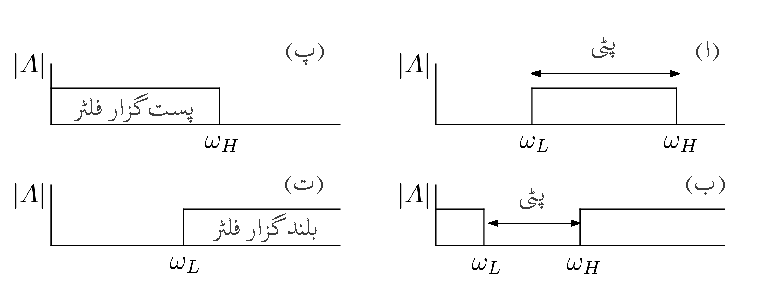
\includegraphics[scale=0.90]{filterDefinition}
\caption{فلٹر کے اقسام}
\label{شکل_تعددی_ردعمل_فلٹر_اقسام}
\end{figure}
%
\حصہ{بٹر ورت فلٹر}
کسی بھی \عددیء{n} درجی تسلسل کو
\begin{align*}
s^n+c_{n-1} s^{n-1}+c_{n-2} s^{n-2}+\cdots+c_2 s^2+c_1 s+c_0
\end{align*}
کی صورت میں لکھا جا سکتا ہے جہاں \عددیء{s=\sigma +j \omega} مخلوط تعدد جبکہ \عددیء{c} تسلسل کے ضربیہ مستقل ہیں۔جفت \عددیء{n} کی صورت میں یعنی \عددیء{n=2,4,6,\cdots} کی صورت میں  
 \عددیء{\left(s^2+2 \zeta_m \omega_m s+\omega_m^2 \right)} طرز کے \عددیء{\tfrac{n}{2}} دو درجی قلیات کو آپس میں ضرب دیتے ہوئے اسی تسلسل کو یوں لکھا جا سکتا ہے
\begin{align}\label{مساوات_تعددی_ردعمل_جفت_تسلسل}
\left(s^2+2 \zeta_1 \omega_1 s+\omega_1^2 \right)\left(s^2+2 \zeta_2 \omega_2 s+\omega_2^2 \right) \cdots
\end{align}
جہاں \عددیء{\zeta_m} اور \عددیء{\omega_m} دو درجی قلیات کے مستقل ہیں۔\عددیء{\zeta_m} کو \موٹا{دھیماپن کا مستقل}\فرہنگ{مستقل!دھیماپن}\حاشیہب{damping constant}\فرہنگ{damping constant} اور \عددیء{\omega_m} کو \موٹا{آزاد قدرتی تعدد}\فرہنگ{قدرتی تعدد!آزاد}\حاشیہب{undamped natural frequency}\فرہنگ{natural frequency!undamped} کہا جاتا ہے۔طاق \عددیء{n} یعنی \عددیء{n=1,3,5,\cdots} کی صورت میں
 \عددیء{\left(s^2+2 \zeta_m \omega_m s+\omega_m^2 \right)} طرز کے \عددیء{\tfrac{n-1}{2}} دو درجی قلیات اور ایک عدد \عددیء{\left(s+\omega_0 \right)} کو آپس میں ضرب دیتے ہوئے اسی تسلسل کو یوں لکھا جا سکتا ہے۔
\begin{align}\label{مساوات_تعددی_ردعمل_طاق_تسلسل}
\left(s+\omega_0 \right)\left(s^2+2 \zeta_1 \omega_1 s+\omega_1^2 \right)\left(s^2+2 \zeta_2 \omega_2 s+\omega_2^2 \right) \cdots
\end{align}

\موٹا{بٹر ورت تسلسل}\فرہنگ{بٹر ورت تسلسل}\حاشیہب{Butterworth}\فرہنگ{Butterworth} \عددیء{B_n(s)} میں مساوات \حوالہ{مساوات_تعددی_ردعمل_جفت_تسلسل} اور مساوات \حوالہ{مساوات_تعددی_ردعمل_جفت_تسلسل} میں تمام \عددیء{\omega_m} برابر ہوتے ہیں۔ایسی صورت میں تمام \عددیء{\omega_m} کو \عددیء{\omega_0} لکھتے ہوئے بٹر ورت تسلسل کو یوں لکھا جا سکتا ہے
\begin{gather}
\begin{aligned}\label{مساوات_تعددی_ردعمل_بٹرورت_تسلسل}
B_n(s)&=\left(s^2+2 \zeta_1 \omega_0 s+\omega_0^2 \right)\left(s^2+2 \zeta_2 \omega_0 s+\omega_0^2 \right) \cdots\\
B_n(s)&=\left(s+\omega_0 \right)\left(s^2+2 \zeta_1 \omega_0 s+\omega_0^2 \right)\left(s^2+2 \zeta_2 \omega_0 s+\omega_0^2 \right) \cdots
\end{aligned}
\end{gather}
جہاں پہلی تسلسل جفت \عددیء{n} اور دوسری تسلسل طاق \عددیء{n} کے لئے ہے۔

آئیں بٹر ورت تسلسل میں \عددیء{s} کی وہ قیمتیں حاصل کریں جن پر \عددیء{B_n(s)} کی قیمت صفر ہو جاتی  ہے۔\عددیء{s} کی یہ قیمتیں تسلسل کے \موٹا{صفر}\فرہنگ{صفر}\حاشیہب{zeros}\فرہنگ{zeros} کہلاتے ہیں۔

\عددیء{s+\omega_0=0} سے \عددیء{s=-\omega_0} حاصل ہوتا ہے۔شکل \حوالہ{شکل_تعددی_ردعمل_بٹر_ورت_تسلسل_کے_صفر} الف میں \موٹا{مخلوط سطح}\فرہنگ{مخلوط سطح}\حاشیہب{complex plane}\فرہنگ{complex plane} پر اس نکتے کو دکھایا گیا ہے۔مخلوط سطح کے افقی محور پر حقیقی اعداد جبکہ اس کے عمودی محور پر خیالی اعداد پائے جاتے ہیں۔یوں \عددیء{s=\sigma+j \omega} لکھتے ہوئے \عددیء{\sigma} کو افقی جبکہ \عددیء{j \omega} کو عمودی محور پر رکھا جائے گا۔

دو درجی قلیات
\begin{align}\label{مساوات_تعددی_ردعمل_دو_درجی_عمومی_جزو}
s^2+2 \zeta_m \omega_0 s +\omega_0^2=0
\end{align}
سے
\begin{gather}
\begin{aligned}
s_1&=s_m =-\zeta_m \omega_0 + j \omega_0 \sqrt{1-\zeta_m^2}\\
s_2&=s_m^* =-\zeta_m \omega_0 - j \omega_0 \sqrt{1-\zeta_m^2}
\end{aligned}
\end{gather}
صفر حاصل ہوتے ہیں۔آپ دیکھ سکتے ہیں کہ کسی بھی دو درجی قلیہ سے دو صفر حاصل ہوتے ہیں جو \عددیء{-\alpha \mp j \beta} کے طرز کے ہوتے ہیں۔اسی لئے انہیں \عددیء{s_m} اور \عددیء{s_m^*} لکھا گیا ہے۔شکل \حوالہ{شکل_تعددی_ردعمل_بٹر_ورت_تسلسل_کے_صفر} ب میں ان صفروں کو دکھایا گیا ہے۔آپ دیکھ سکتے ہیں کہ دونوں صفر عمودی محور کے بائیں جانب پائے جاتے ہیں۔ایک صفر افقی محور کے اوپر جانب جبکہ دوسرا صفر محور کے نیچھے جانب پایا جاتا ہے۔دونوں افقی محور سے برابر فاصلے پر پائے جاتے ہیں۔یہ  عمومی نتائج ہیں۔

\عددیء{s_m} اور \عددیء{s_m^*} کی حتمی قیمت
\begin{align}
\abs{s_m}=\abs{s_m^*}=\omega_0
\end{align}
حاصل ہوتی ہے۔کسی بھی مخلوط عدد کو حقیق اور خیالی اجزاء کی صورت میں لکھا جا سکتا ہے۔اسی مخلوط عدد کو حتمی قیمت اور زاویے کی شکل میں بھی لکھا جا سکتا ہے۔یوں \عددیء{s_m} مخلوط عدد کو مثال بناتے ہوئے اسے دونوں طرح لکھتے ہیں۔
\begin{align}
s_m=-\zeta_m \omega_0 +j \omega_0 \sqrt{1-\zeta_m^2}= \abs {s_m} \phase \theta
\end{align}
جہاں
\begin{align}\label{مساوات_تعددی_ردعمل_صفر_حتمی_فاصلہ}
\abs{s_m}&=\sqrt{\zeta_m^2 \omega_0^2 +\omega_0^2\left(1 -\zeta_m^2\right)}=\omega_0
\end{align}
کے برابر ہے۔شکل \حوالہ{شکل_تعددی_ردعمل_بٹر_ورت_تسلسل_کے_صفر} ب میں نکتہ  \عددیء{s_m} سے  نکتہ \عددیء{o} تک کا فاصلہ \عددیء{\abs{s_m}} یعنی اس کی حتمی قیمت دکھلاتا ہے۔اس شکل میں زاویہ \عددیء{\phase{\theta_m}} دکھایا گیا ہے۔شکل کو دیکھتے ہوئے
\begin{align}\label{مساوات_تعددی_ردعمل_دھیماپن_کا_حصول}
\cos \theta_m=\frac{\zeta_m \omega_0}{\omega_0}=\zeta_m
\end{align}
لکھا جا سکتا ہے۔

مساوات \حوالہ{مساوات_تعددی_ردعمل_صفر_حتمی_فاصلہ} کے تحت تمام صفروں کی حتمی قیمت \عددیء{\omega_0} کے برابر ہے۔یوں مخلوط سطح پر تمام صفر  \عددیء{\omega_0} رداس کے دائرے پر پائے جائیں گے۔اس حقیقت کو شکل \حوالہ{شکل_تعددی_ردعمل_بٹر_ورت_تسلسل_کے_صفر} پ میں دکھایا گیا ہے۔آپ دیکھ سکتے ہیں کہ \عددیء{s_1} اور \عددیء{s_1^*} آپس میں افقی محور کے الٹ جانب برابر فاصلے پر ہیں۔یہی کچھ \عددیء{s_2} اور \عددیء{s_2^*} کے لئے بھی درست ہے۔بٹر ورت تسلسل کے تمسام صفر اسی دائرے پر عمودی محور کے بائیں جانب پائے جائیں گے۔ 
\begin{figure}
\centering
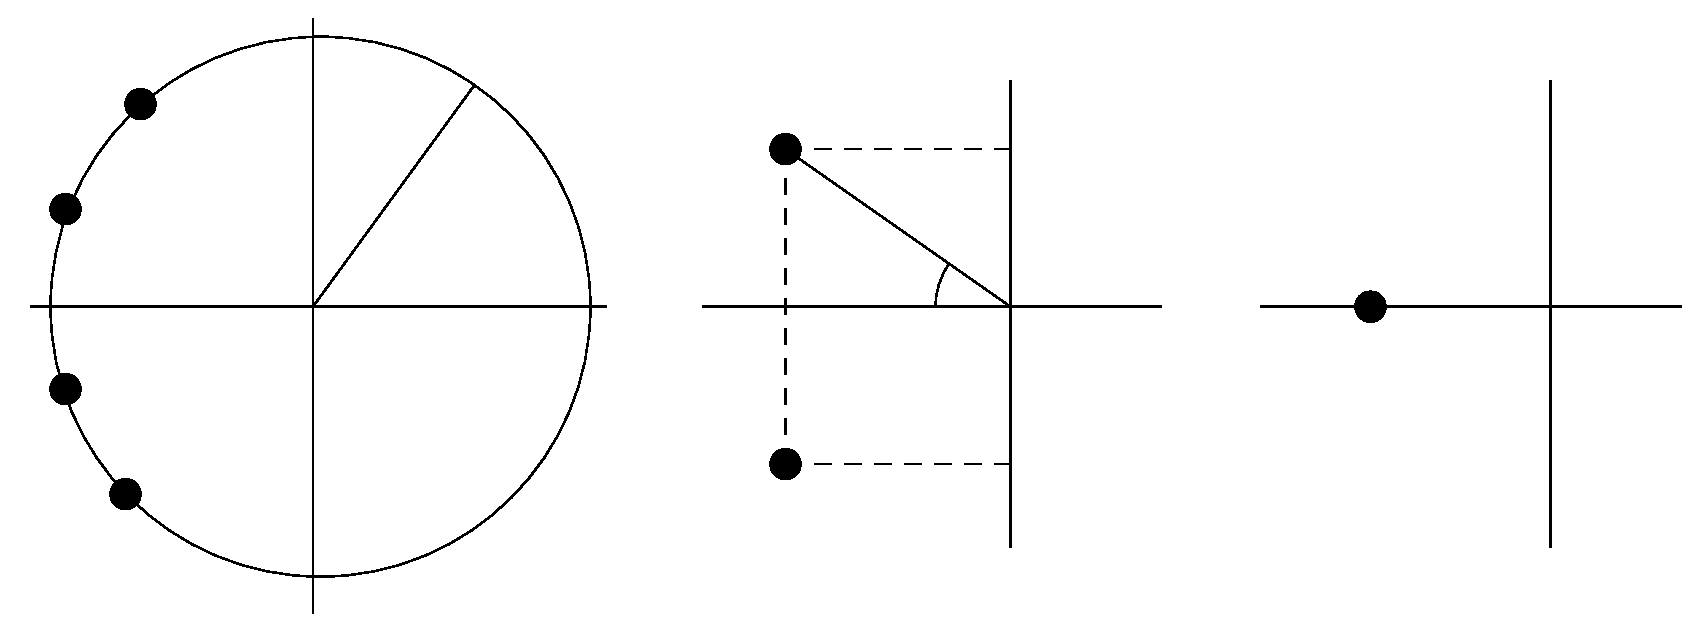
\includegraphics[scale=0.90]{butterworthCircleComplexPlane}
\caption{مخلوط سطح پر بٹر ورت  تسلسل کے صفر}
\label{شکل_تعددی_ردعمل_بٹر_ورت_تسلسل_کے_صفر}
\end{figure}

بٹر ورت تسلسل کے کسی بھی دو درجی جزو کو
\begin{align*}
s^2+s \zeta_m \omega_0 s+\omega_0^2=\omega_0^2 \left[\left(\frac{s}{\omega_0} \right)^2 +2 \zeta_m \left(\frac{s}{\omega_0} \right)+1\right]
\end{align*}
کی صورت میں لکھا جا سکتا ہے۔اگر  مساوات \حوالہ{مساوات_تعددی_ردعمل_دو_درجی_عمومی_جزو} میں \عددیء{\omega_0=1} رکھا جاتا تب شکل \حوالہ{شکل_تعددی_ردعمل_بٹر_ورت_تسلسل_کے_صفر} پ میں دائرے کا رداس ایک کے برابر ہوتا جبکہ مساوات \حوالہ{مساوات_تعددی_ردعمل_دھیماپن_کا_حصول} اب بھی  درست ثابت ہوتا۔اکائی رداس کے اس دائرے کو \موٹا{بٹر ورت دائرہ}\فرہنگ{بٹر ورت دائرہ}\حاشیہب{Butterworth circle}\فرہنگ{Butterworth circle}  کہا جائے گا۔

\موٹا{بٹر ورت فلٹر}\فرہنگ{فلٹر!بٹر ورت}\حاشیہب{Butterworth filter}\فرہنگ{filter!Butterworth} کا عمومی قلیہ
\begin{align}\label{مساوات_تعددی_ردعمل_بٹرورت_پست_گزار}
A(s)=\frac{A_0}{B_n(s)}
\end{align}
ہے۔اس مساوات کی حتمی قیمت نہایت سادہ شکل رکھتی ہے۔
\begin{align}
\abs{A(s)}=\frac{\abs{A_0}}{\sqrt{1+\left(\frac{\omega}{\omega_0} \right)^{2n}}}
\end{align}
\عددیء{\abs{A_0}=1} لیتے ہوئے \عددیء{\abs{A(s)}} کے خط کو \عددیء{n} کی مختلف قیمتوں کے لئے شکل \حوالہ{شکل_تعددی_ردعمل_بٹر_ورت_پست_گزار} میں کھینچا گیا ہے۔آپ دیکھ سکتے ہیں کہ \عددیء{n} کی تمام قیمتوں کے لئے \عددیء{\abs{A}} کی قیمت \عددیء{\omega_0} تعدد پر \عددیء{\SI{3}{\deci \bel}} گٹھ جاتی ہے۔ساتھ ہی ساتھ یہ حقیقت بھی واضح ہے کہ \عددیء{n} کی  قیمت بڑھانے سے شکل \حوالہ{شکل_تعددی_ردعمل_بٹر_ورت_پست_گزار} کی صورت  شکل \حوالہ{شکل_تعددی_ردعمل_فلٹر_اقسام} پ کے قریب تر ہوتی جاتی ہے۔ 
\begin{figure}
\centering
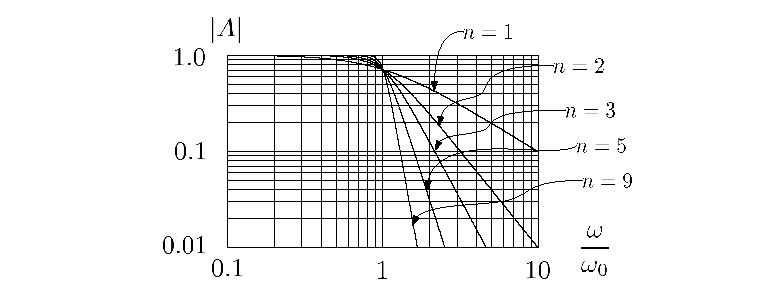
\includegraphics[scale=0.90]{butterworthFilterLowPassResponse}
\caption{بٹر ورت پست گزار فلٹر}
\label{شکل_تعددی_ردعمل_بٹر_ورت_پست_گزار}
\end{figure}

\عددیء{\omega_0=1} کی صورت میں بٹر ورت کے تسلسل کو جدول \حوالہ{جدول_تعددی_ردعمل_بٹرورت_قلیات} میں پیش کیا گیا ہے۔طاق \عددیء{n} کی صورت میں بٹر ورت تسلسل میں \عددیء{\left(s+1 \right)} پایا جاتا ہے جبکہ جفت \عددیء{n} کی صورت میں صرف  دو درجی\حاشیہب{quadratic} اجزاء پائے جاتے ہیں۔
 
\begin{table}
\caption{بٹر ورت تسلسل}
\label{جدول_تعددی_ردعمل_بٹرورت_قلیات}
\centering
\begin{tabular}{l l}
\toprule
$B_n(s)$&$n$\\
\midrule
$\left(s+1 \right) $ &1\\
$ \left(s^2+1.414s+1 \right)$&2\\
$\left(s+1\right)\left(s^2+s+1 \right)$ &3\\
$\left(s^2+0.765s+1\right)\left(s^2+1.848s+1\right)$&4\\
$\left(s+1\right)\left(s^2+0.618s+1\right)\left(s^2+1.618s+1\right)$&5\\
$\left(s^2+0.518s+1 \right)\left(s^2+1.414s+1\right)\left(s^2+1.932s+1\right)$&6\\
\bottomrule
\end{tabular}
\end{table}
%
بٹر ورت تسلسل میں \عددیء{\omega_0=1} لیتے ہوئے دو درجی اجزاء کو \عددیء{\left(s^2+2 \zeta s +1 \right)} لکھا جا سکتا ہے جہاں \عددیء{\zeta} کو بٹر ورت دائرے  سے حاصل کیا جا سکتا ہے۔شکل \حوالہ{شکل_تعددی_ردعمل_بٹر_ورت_دائرہ_جفت} میں بٹر ورت دائرے سے جفت \عددیء{n} کی صورت میں \عددیء{\zeta} کا حصول دکھایا گیا ہے۔بٹر ورت دائرے کا رداس\حاشیہب{radius} ایک کے برابر ہے۔جفت \عددیء{n} کی صورت میں اس دائرے پر زاویہ \عددیء{\phase{aoa'}} کھینچا  جاتا ہے جہاں یہ زاویہ  \عددیء{\tfrac{\pi}{n}} کے برابر ہوتا ہے۔یوں \عددیء{n=2} کی صورت میں اس دائرے پر \عددیء{\tfrac{\pi}{2}} یعنی \عددیء{\SI{90}{\degree}} کا زیویہ کھینچا جائے گا۔اس زاویے کو یوں کھینچا جاتا ہے کہ \عددیء{\phase{aoo'}=\phase{a'oo'}} ہوں۔شکل \حوالہ{شکل_تعددی_ردعمل_بٹر_ورت_دائرہ_جفت} الف میں ایسا کیا گیا ہے۔\عددیء{\phase{aoo'}} کو \عددیء{\theta} لکھتے ہوئے \عددیء{\zeta} کو
\begin{align}
\zeta=\cos \theta
\end{align}
سے حاصل کیا جاتا ہے۔یوں \عددیء{n=2} کی صورت میں
\begin{align*}
\zeta=\cos 45=0.7071
\end{align*}
حاصل ہوتا ہے اور بٹر ورت قلیہ
\begin{align*}
s^2+2 \zeta s+1=s^2+1.4142s+1
\end{align*}
صورت اختیار کر لیگا جو جدول \حوالہ{جدول_تعددی_ردعمل_بٹرورت_قلیات} کے عین مطابق ہے۔
\begin{figure}
\centering
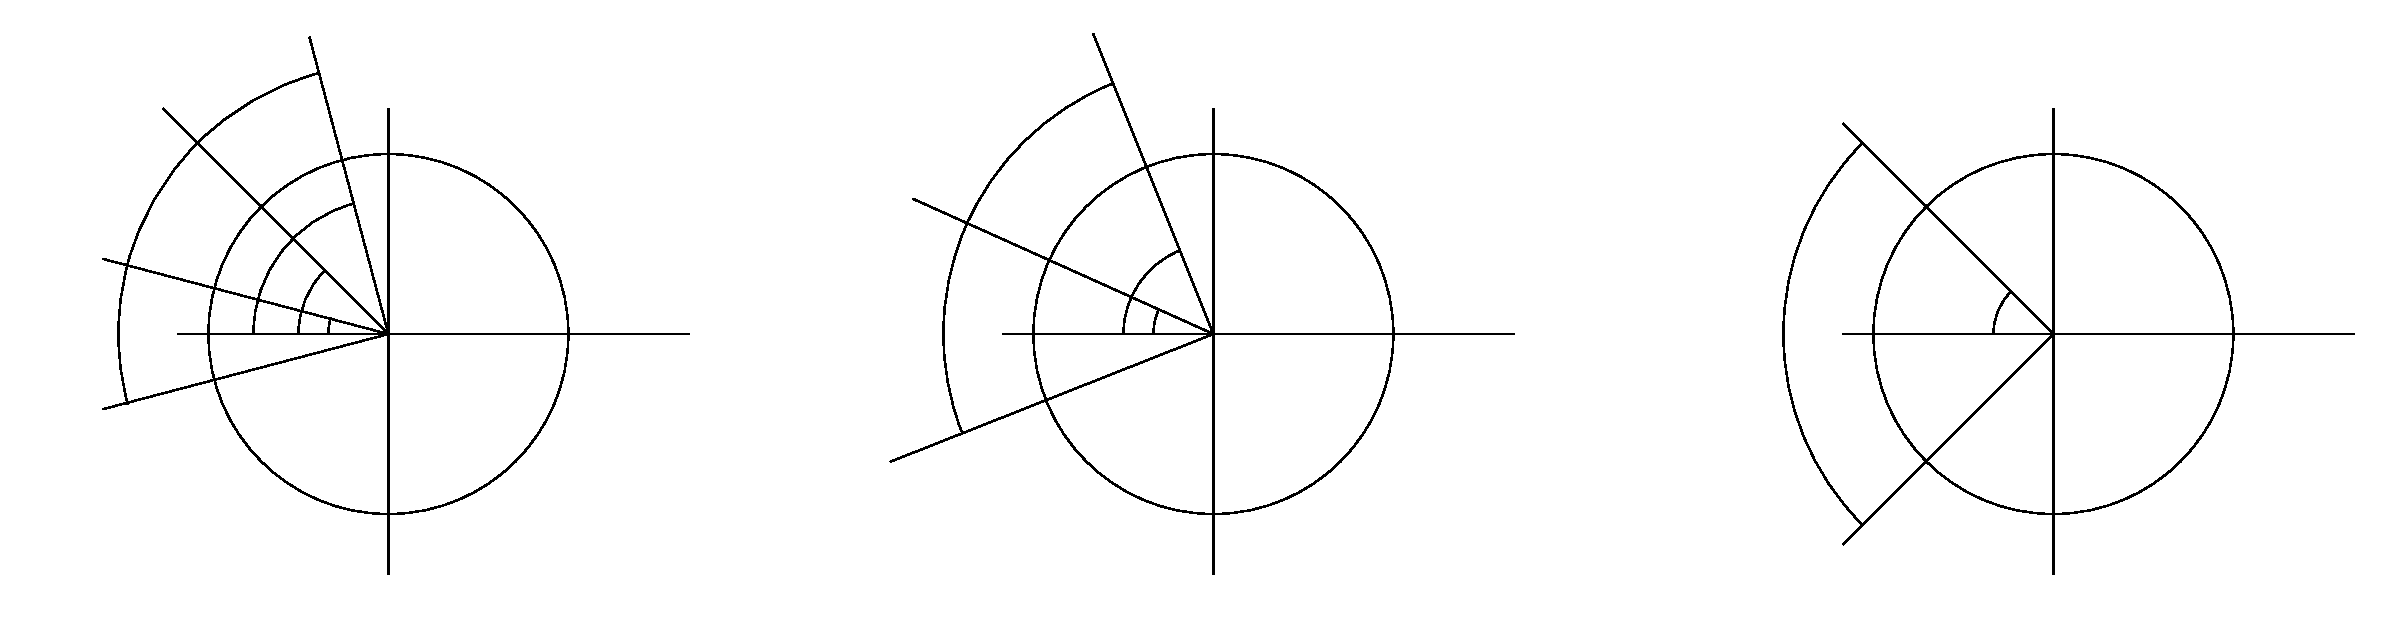
\includegraphics[scale=0.90]{butterworthCircle}
\caption{جفت بٹر ورت دائرہ}
\label{شکل_تعددی_ردعمل_بٹر_ورت_دائرہ_جفت}
\end{figure}

شکل \حوالہ{شکل_تعددی_ردعمل_بٹر_ورت_دائرہ_جفت} ب میں \عددیء{n=4} ہے۔
یوں \عددیء{\phase{aoa'}=\tfrac{\pi}{4}=\SI{45}{\degree}} ہو گا جہاں \عددیء{\phase{aoo'}=\phase{a'oo'}} ہی رکھے گئے ہیں۔\عددیء{n=4} کی  صورت میں بٹر ورت قلیے میں دو درجی اجزاء دو مرتبہ پائے جاتے ہیں۔یوں ایک اضافی زاویہ \عددیء{\phase{aob}=\SI{45}{\degree}} بھی کھینچا جاتا ہے۔یوں
\begin{align*}
\theta_1&=\phase{aoo'}=\SI{22.5}{\degree}\\
\theta_2&=\phase{boo'}=\SI{67.5}{\degree}
\end{align*}
ہوں گے جن سے
\begin{align*}
\zeta_1&=\cos 22.5=0.9239\\
\zeta_2&=\cos 67.5=0.3827
\end{align*}
حاصل ہوتے ہیں لہٰذا بٹر ورت قلیہ
\begin{align*}
\left(s^2+2 \times 0.9239 \times s +1\right) \left(s^2+2 \times 0.3827s+1 \right)
\end{align*}
یعنی
\begin{align*}
\left(s^2+1.848s \right) \left(s^2+0.765s+1 \right)
\end{align*}
ہو گا۔
%
\begin{figure}
\centering
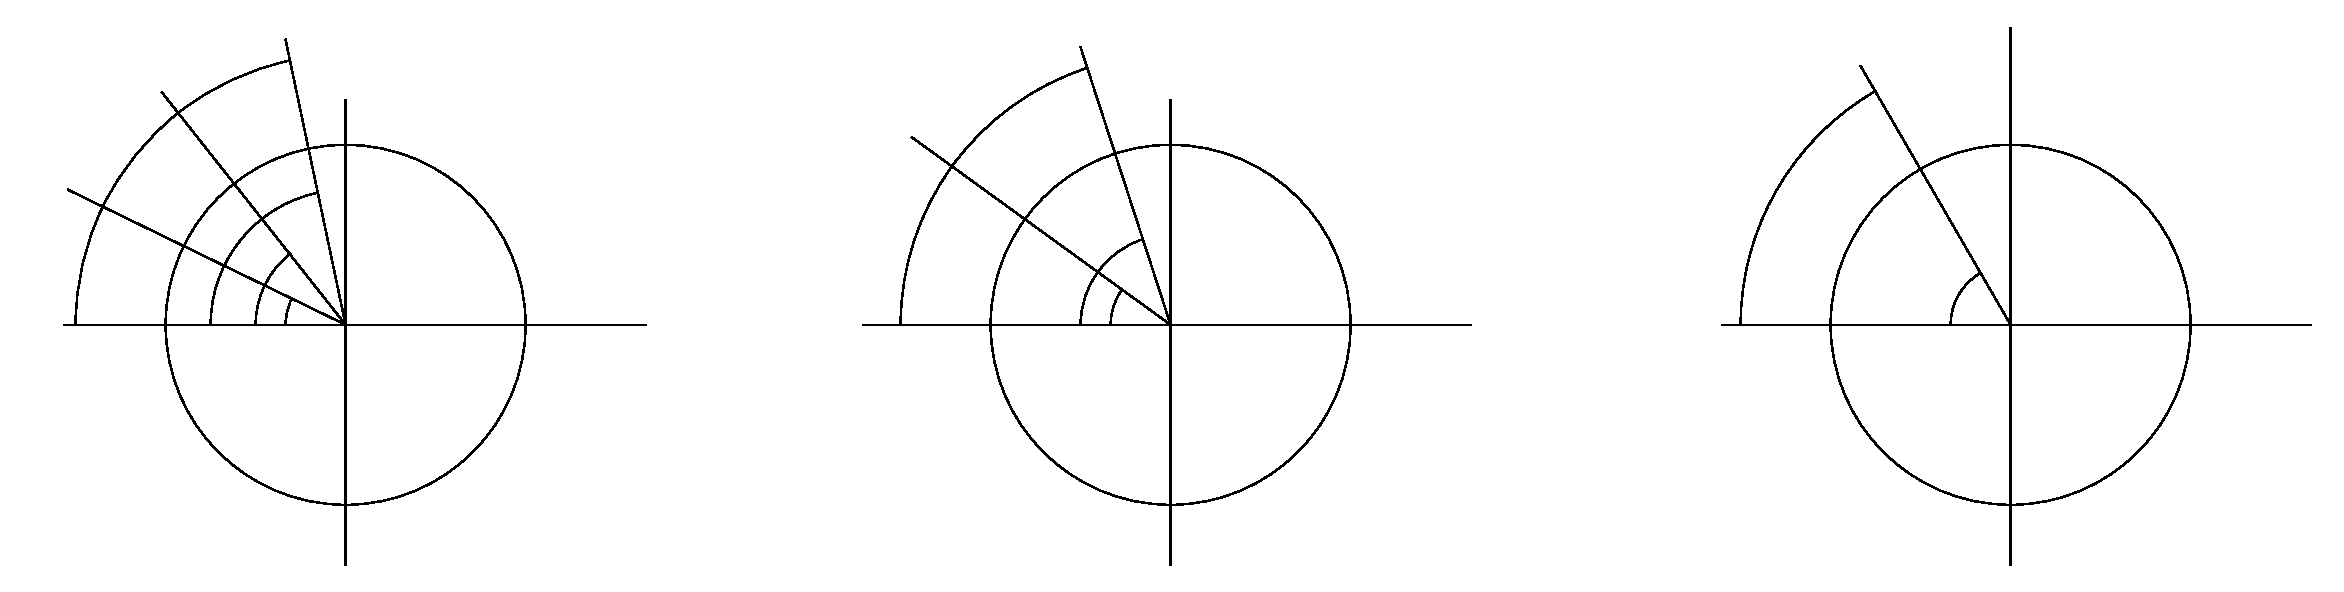
\includegraphics[scale=0.90]{butterworthCircleOdd}
\caption{طاق بٹر ورت دائرہ}
\label{شکل_تعددی_ردعمل_بٹر_ورت_دائرہ_طاق}
\end{figure}
شکل \حوالہ{شکل_تعددی_ردعمل_بٹر_ورت_دائرہ_طاق} میں طاق \عددیء{n} کی صورت میں \عددیء{\theta} کا حصول دکھایا گیا ہے۔شکل-الف میں \عددیء{n=3} کے لئے حل کیا گیا ہے جہاں \عددیء{\phase{aoo'}} کا زاویہ \عددیء{\tfrac{\pi}{n}} یعنی \عددیء{\SI{60}{\degree}} کا کھینچا گیا ہے۔\عددیء{\theta=\phase{aoo'}} لیتے ہوئے
\begin{align*}
\zeta=\cos 60=0.5
\end{align*}
حاصل ہوتا ہے۔طاق بٹر ورت قلیے میں \عددیء{\left(s+1 \right)} کا اضافی جزو پایا جاتا ہے لہٰذا \عددیء{n=3} کی صورت میں بٹر ورت قلیہ
\begin{align*}
\left(s+1 \right)\left(s^2+2 \times 0.5 \times s+ 1\right)
\end{align*}
یعنی
\begin{align*}
\left(s+1 \right)\left(s^2+ s+1 \right)
\end{align*}
ہو گا۔\عددی{n=5} کی صورت میں \عددیء{\phase{aoo'}=\tfrac{\pi}{5}} یعنی \عددیء{\SI{36}{\degree}} کھینچنے کے بعد \عددیء{\phase{boa}} بھی \عددیء{\SI{36}{\degree}} کھینچیں۔یوں
\begin{align*}
\theta_1&=\phase{aoo'}\\
\theta_2&=\phase{boo'}
\end{align*}
ہوں گے۔

جدول \حوالہ{جدول_تعددی_ردعمل_بٹرورت_قلیات} میں \عددیء{\omega_0 \ne 1} لیتے ہوئے پہلے درجے  بٹر ورت فلٹر کے قلیہ کو
\begin{align}\label{مساوات_تعددی_بٹرورت_پہلا_درجہ}
\frac{A(s)}{A_0}=\frac{1}{\left(\frac{s}{\omega_0}\right)+1}
\end{align}
جبکہ دو درجی بٹر ورت فلٹر کے قلیہ کو
\begin{align}\label{مساوات_تعددی_بٹرورت_دوسرا_درجہ}
\frac{A(s)}{A_0}=\frac{1}{\left(\frac{s}{\omega_0} \right)^2+2 \zeta \left(\frac{s}{\omega_0} \right)+1}
\end{align}
لکھا جا سکتا ہے۔

\جزوحصہ{بٹر ورت فلٹر کا دور}
شکل \حوالہ{شکل_تعددی_ردعمل_بٹر_ورت_فلٹر_دور} الف میں
\begin{align*}
v_k&=\left(\frac{\frac{1}{sC}}{R+\frac{1}{sC}} \right) v_i=\frac{v_i}{sRC+1}\\
v_o&=\left(1+\frac{R_2}{R_1} \right)v_k
\end{align*}
لکھا جا سکتا ہے جس سے
\begin{align*}
A(s) =\frac{v_o}{v_i}&=\left(1+\frac{R_2}{R_1} \right)\left(\frac{1}{sRC+1}\right)
\end{align*}
حاصل ہوتا ہے۔اس میں
\begin{align*}
\omega_0&=\frac{1}{RC}\\
A_0&=1+\frac{R_2}{R_1}
\end{align*}
لکھتے ہوئے
\begin{align*}
\frac{A(s)}{A_0}=\frac{1}{\left(\frac{s}{\omega_0}\right)+1}
\end{align*}
حاصل ہوتا ہے۔اس کا مساوات \حوالہ{مساوات_تعددی_بٹرورت_پہلا_درجہ} کے ساتھ سے موازنا کریں جو پہلے درجے کی بٹر ورت فلٹر کی مساوات ہے۔آپ دیکھ سکتے ہیں کہ شکل \حوالہ{شکل_تعددی_ردعمل_بٹر_ورت_فلٹر_دور} الف پہلے درجے کا بٹر ورت فلٹر ہے۔
\begin{figure}
\centering
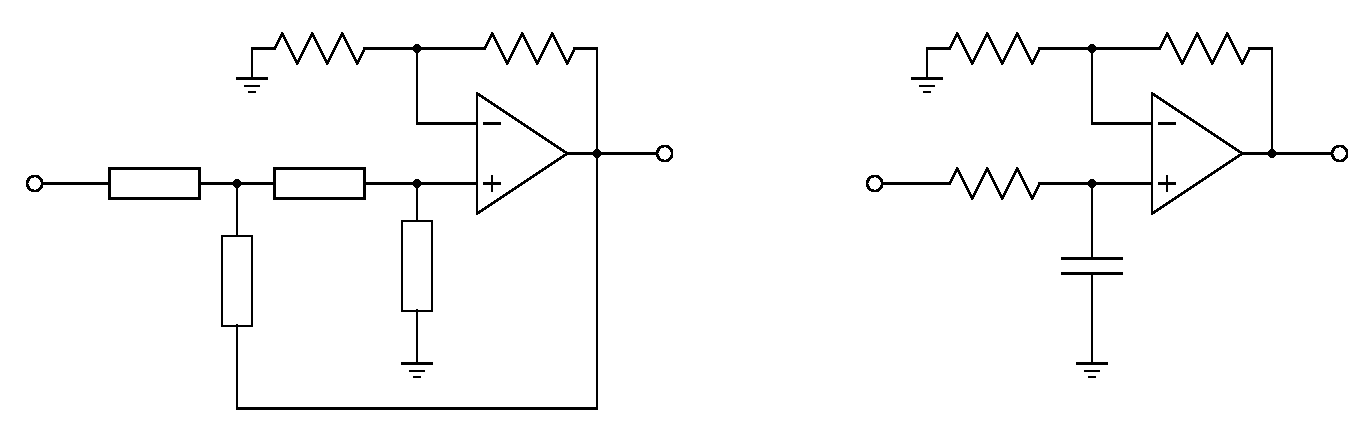
\includegraphics[scale=0.90]{butterworthImplementation}
\caption{بٹر ورت فلٹر}
\label{شکل_تعددی_ردعمل_بٹر_ورت_فلٹر_دور}
\end{figure}
%

آئیں شکل \حوالہ{شکل_تعددی_ردعمل_بٹر_ورت_فلٹر_دور} ب میں دئے دوسرے درجے کے بٹر ورت فلٹر کو حل کریں۔جوڑ \عددیء{v_1} پر کرچاف کے قانون برائے برقی رو کی مدد سے
\begin{align*}
\frac{v_1-v_i}{Z_1}+\frac{v_1}{Z_3+Z_4}+\frac{v_1-v_o}{Z_2}=0
\end{align*}
لکھا جا سکتا ہے جبکہ کرچاف کے قانون برائے برقی دباو کی مدد سے 
\begin{align*}
v_k= \left(\frac{Z_4}{Z_3+Z_4} \right) v_1
\end{align*}
لکھا جا سکتا ہے۔مثبت ایمپلیفائر کے لئے
\begin{align*}
v_o=\left(1+\frac{R_2}{R_1}\right) v_k=A_0 v_k
\end{align*}
لکھا جا سکتا ہے۔ان تینوں مساوات کو حل کرنے سے
\begin{align}\label{مساوات_تعددی_دو_درجی_بٹرورت_فلٹر_کی_افزائش}
A(s)=\frac{v_o}{v_i}=\frac{A_0 Z_2 Z_4}{Z_2 \left(Z_1+Z_3+Z_4 \right)+Z_1 Z_4 \left(1-A_0 \right)}
\end{align}
حاصل ہوتا ہے۔پست گزار فلٹر کی صورت میں \عددیء{Z_1} اور \عددیء{Z_3} مزاحمت جبکہ \عددیء{Z_2} اور \عددیء{Z_4} کپیسٹر ہوتے ہیں۔ایسا دور شکل \حوالہ{شکل_تعددی_ردعمل_بٹر_ورت_فلٹر_پست_بلند_گزار} الف میں دکھایا گیا ہے۔اس کے برعکس بلند گزار فلٹر میں \عددیء{Z_1} اور \عددیء{Z_3} کپیسٹر جبکہ \عددیء{Z_2} اور \عددیء{Z_4} مزاحمت ہوتے ہیں۔شکل \حوالہ{شکل_تعددی_ردعمل_بٹر_ورت_فلٹر_پست_بلند_گزار} ب میں بلند گزار فلٹر دکھایا گیا ہے۔  
\begin{figure}
\centering
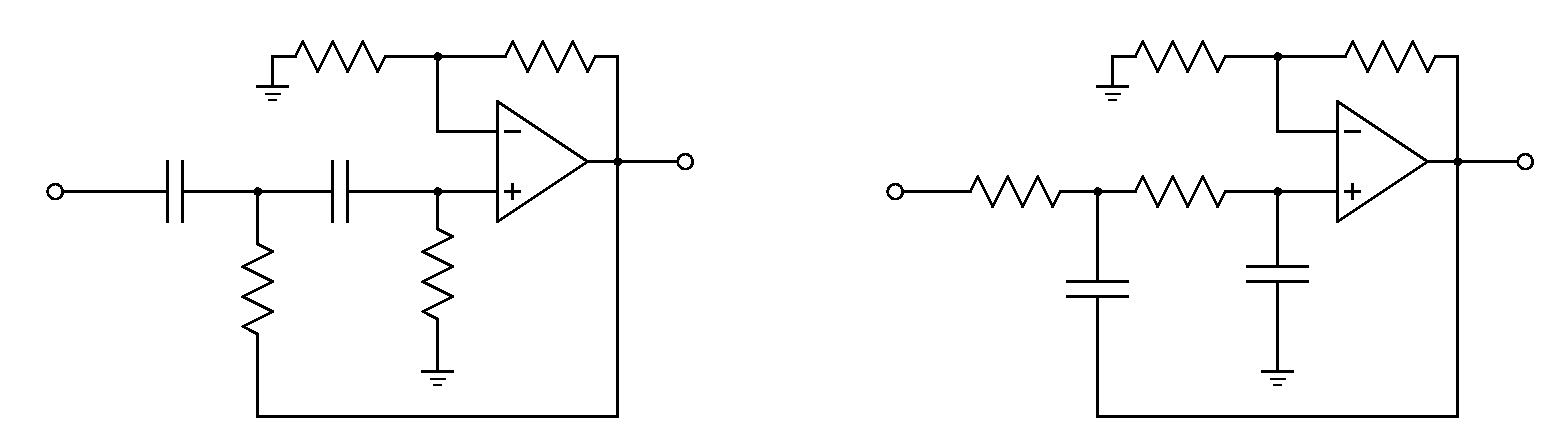
\includegraphics[scale=0.90]{butterworthLowPassFilterImplementation}
\caption{بٹر ورت پست گزار اور بلند گزار فلٹر}
\label{شکل_تعددی_ردعمل_بٹر_ورت_فلٹر_پست_بلند_گزار}
\end{figure}

شکل \حوالہ{شکل_تعددی_ردعمل_بٹر_ورت_فلٹر_پست_بلند_گزار} الف کے لئے مساوات \حوالہ{مساوات_تعددی_دو_درجی_بٹرورت_فلٹر_کی_افزائش}
\begin{align}\label{مساوات_تعددی_دو_درجی_بٹرورت_پست_گزار_فلٹر_کی_افزائش}
A(s)=\frac{A_0 \left(\frac{1}{RC} \right)^2}{s^2+\left(\frac{3-A_0}{RC} \right) s+ \left(\frac{1}{RC} \right)^2}
\end{align}
مساوات \حوالہ{مساوات_تعددی_دو_درجی_بٹرورت_پست_گزار_فلٹر_کی_افزائش} کا مساوات \حوالہ{مساوات_تعددی_بٹرورت_دوسرا_درجہ} کے ساتھ موازنا کرتے ہوئے
\begin{gather}
\begin{aligned}
\omega_0&=\frac{1}{RC}\\
A_0&=3-2 \zeta
\end{aligned}
\end{gather}
حاصل ہوتے ہیں۔

ان معلومات کے ساتھ اب ہم بٹر ورت فلٹر تخلیق دے سکتے ہیں۔\عددیء{RC} کو درکار \عددی{\tfrac{1}{\omega_0}} کے برابر رکھا جاتا ہے جہاں پست گزار فلٹر کی صورت میں یہ \عددیء{\omega_H} جبکہ بلند گزار فلٹر کی صورت میں \عددیء{\omega_0=\omega_L} کے برابر ہو گا۔جفت \عددیء{n} کی صورت میں شکل \حوالہ{شکل_تعددی_ردعمل_بٹر_ورت_فلٹر_پست_بلند_گزار} الف طرز کے \عددیء{\tfrac{n}{2}} کڑیاں استعمال کرتے ہوئے زنجیری ایمپلیفائر بنایا جاتا ہے۔جدول \حوالہ{جدول_تعددی_ردعمل_بٹرورت_قلیات} سے مطلابہ دو درجی قلیات کے \عددیء{\zeta} حاصل کئے جاتے ہیں۔ہر \عددیء{\zeta} کے لئے ایک کڑی تخلیق دی جاتی ہے۔طاق \عددیء{n} کی صورت میں شکل \حوالہ{شکل_تعددی_ردعمل_بٹر_ورت_فلٹر_پست_بلند_گزار} الف کے طرز پر \عددیء{\tfrac{n-1}{2}} کڑیوں کے علاوہ شکل \حوالہ{شکل_تعددی_ردعمل_بٹر_ورت_فلٹر_دور} الف کے طرز پر اضافی کڑی بھی استعمال کی جاتی ہے۔
